\section{Fordeling af besvarelser}
\label{TestAfSkalaFordeling}
%
I følgende afsnit vil fordelingen af besvarelserne blive præsenteret. Dette dækker over den gennemsnitlige besvarelse til hver af de 23 skalaer samt eksempler på forskellige fordelinger, der er med til at illustrere, at der eksisterer stor varians på tværs af besvarelserne. Til sidst vil data blive præsenteret i et boksplot og diskuteret.
%
\begin{figure}[H]
\centering
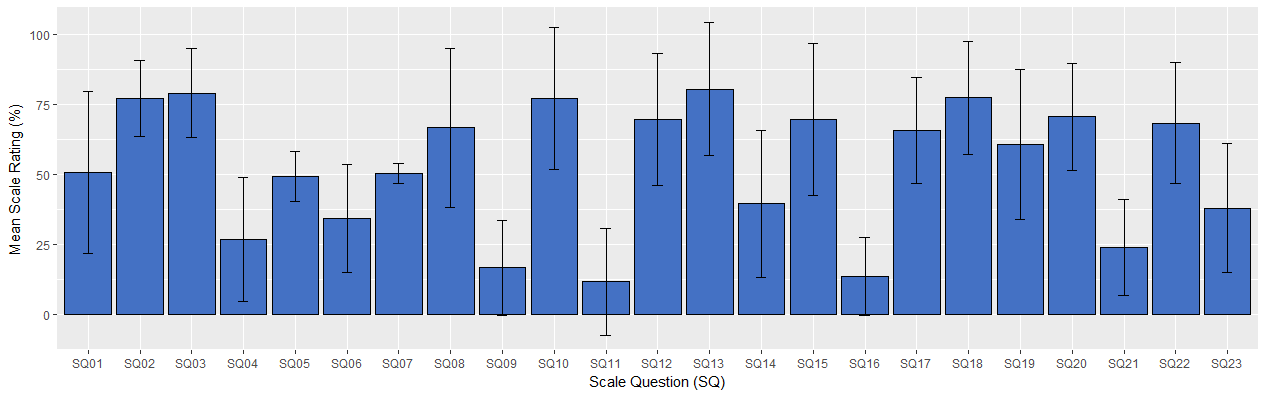
\includegraphics[width = \textwidth]{Figure/DatabehandlingSkalaer/DataPresentation/MeanBarplot} 
 \caption{Søjlediagram over den gennemsnitlige besvarelse (\%) til hvert skalaspørgsmål (SQ) samt barer, der repræsenterer standardafvigelsen for hver SQ.}
\label{fig:BarPlotGennemsnit}
\end{figure}
\noindent
%
På \autoref{fig:BarPlotGennemsnit} er det tydeligt, at der forekommer stor variation mellem besvarelserne til de enkelte skalaspørgsmål, dog med undtagelse af SQ7 vedrørende robottens højde og tildels SQ5 vedrørende robottens afstand. Der er udarbejdet et kombineret histogram og normalfordelingsplot for hver skala, for at få en mere nøjagtig indsigt i, hvordan besvarelserne er fordelt. Enkelte af dem vil blive beskrevet i dette afsnit, mens resten fremgår af \fullref{ElektroniskBilagHistNormal}.
%
\begin{figure}[H]
\centering
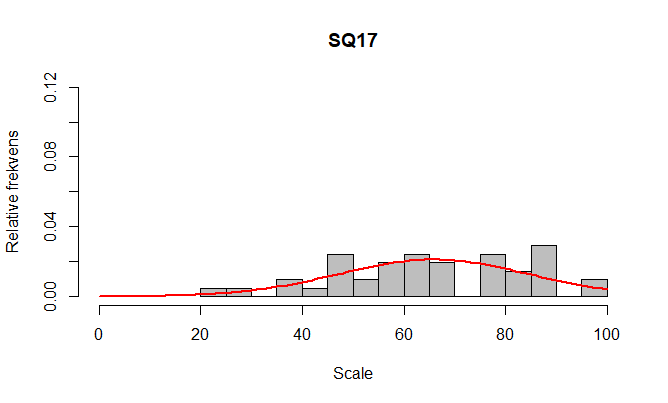
\includegraphics[width = \textwidth]{Figure/DatabehandlingSkalaer/HistogramNormalFordeling/SQ17} 
\caption{Fordelingerne af besvarelserne til SQ17, vedrørende hvor elegant robotten er. Histogrammet repræsenterer hyppigheden af besvarelser (y-aksen) målt som relativ frekvens (Antal/SampleSize), inden for de fastsatte intervaller (x-aksen), angivet i \%. Den sorte kurve repræsenterer den underliggende normalfordelingskurve, som er baseret på middelværdien og standardafvigelsen.}
\label{fig:Histogram17}
\end{figure}
\noindent
%
\autoref{fig:Histogram17} repræsenterer histogrammet for SQ17, vedrørende hvor elegant robotten er, med tilhørende normalfordelingskurve og er et eksempel på hvordan resten af histogrammerne er visualiseret. Da en stor del af data befinder sig under den sorte kurve, tyder det på, at besvarelserne for SQ17 er tilnærmelsesvist normalfordelte. Dette undersøges dog ikke med en signifikanstest, \textit{Shapiro-Wilk Normality Test}, da formålet med gennemgangen blot er at få et overblik over fordelingerne.\blankline
%
Normalfordelings kurverne i flere af plottene forekommer meget flade, hvilket skyldes, at akserne holdes konstante på tværs af plottene, for bedre at kunne sammenligne dem indbyrdes. Dette er dog med undtagelse af histogrammer og normalfordelinger for SQ5, SQ7 og SQ11, da data er meget centreret omkring midten og til venstre på disse histogrammer. Det kan derfor være svært at se fordelingerne på de resterende histogrammer, hvis akserne defineres ud fra SQ5, SQ7 og SQ11.\blankline
%
I mange af plottene er der en stor varians, hvilket indikerer at en stor del af skalaen er blevet anvendt. Her skal det tilføjes at besvarelserne er givet ud fra forskellige højder, afstande og indgangsvinkler og at variationen derfor ikke nødvendigvis er et udtryk for at testpersonerne er uenige, men snarere at de har vurderet forskellige stimuli. Et eksempel er givet på \autoref{fig:Histogram14}.\blankline
%
\begin{figure}[H]
\centering
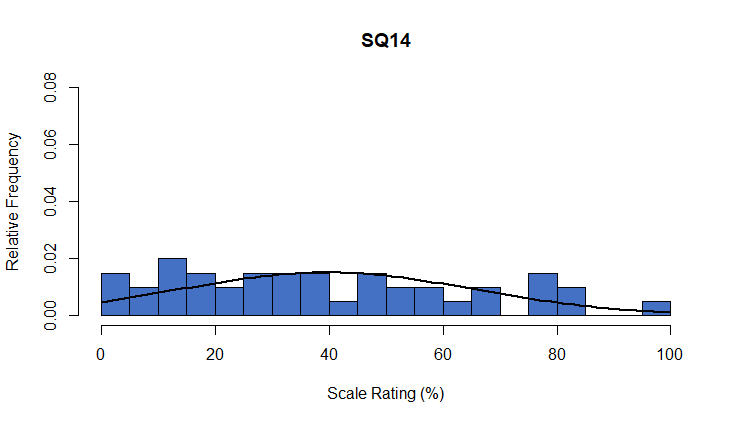
\includegraphics[width = \textwidth]{Figure/DatabehandlingSkalaer/HistogramNormalFordeling/SQ14} 
\caption{Fordelingerne af besvarelserne til SQ14, vedrørende hvor personlig robottens hjælp opleves. Histogrammet repræsenterer hyppigheden af besvarelser (y-aksen) målt som relativ frekvens (Antal/SampleSize), inden for de fastsatte intervaller (x-aksen), angivet i \%. Den sorte kurve repræsenterer den underliggende normalfordelingskurve, som er baseret på middelværdien og standardafvigelsen.}
\label{fig:Histogram14}
\end{figure}
\noindent
%
I disse histogram- og normalfordelingsplots fokuseres der på, hvordan besvarelserne er fordelt for hvert enkelt skalaspørgsmål, men for at få et samlet overblik, fokuseres der på \autoref{fig:Boksplots}. 
%
\begin{figure}[H]
\centering
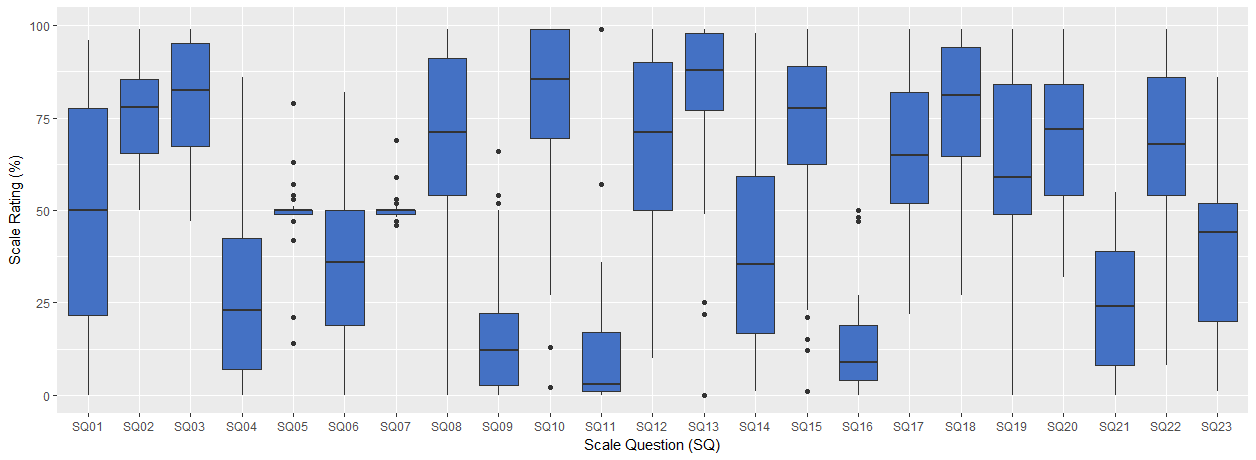
\includegraphics[width = \textwidth]{Figure/DatabehandlingSkalaer/BoksplotUden0er} 
\caption{Boksplot over fordelinger af besvarelserne (angivet i \% på y-aksen) for hvert skalaspørgsmål (angivet med \textit{SQ} på x-aksen). De manglende besvarelser er ekskluderet fra dette boksplot, så det udelukkende bygger på reelle besvarelser.}
\label{fig:Boksplots}
\end{figure}
\noindent
%
\autoref{fig:Boksplots} deler alle besvarelserne til det pågældende skalaspørgsmål op i fire kvartiler. Medianen adskiller det interkvartile område, som repræsenterer 50 \% af data, og kanterne på det interkvartile område adskiller disse fra de to yderste kvartiler. Outliers er ikke medregnet i kvartilerne for boksplottet, men er stadig plottet for at give en idé om hvordan de fordeler sig i forhold til resten af besvarelserne. \blankline
%
Ud fra \autoref{fig:Boksplots} fremgår det, at fordelingerne adskiller sig fra hinanden. Testpersonerne udnytter en stor del af nogle af skalaerne (SQ1, SQ4, SQ8, SQ12, SQ14, SQ19, SQ22, SQ23), hvorimod besvarelserne på andre skalaer fordeler sig over mindre områder, hvilket gør sig gældende for: SQ2, SQ3, SQ5, SQ7, SQ9, SQ11, SQ13 og SQ16. Nogle boksplot gengiver tilnærmelsesvis en normalfordeling, (SQ1, SQ2, SQ6, SQ17, SQ20, SQ21), mens andre er skævevredet den ene eller anden vej (SQ8, SQ9, SQ10, SQ11, SQ13, SQ18). Der forekommer også enkelte boksplots, hvor datapunkterne ophober sig omkring endepunkterne eller midtpunktet (SQ5, SQ7, SQ9, SQ10, SQ11, SQ13). \blankline
%
Den lave varians, som forekommer i nogle af boksplottene, kan skyldes forskellige ting. Det kan enten skyldes, at parameteren ikke er vigtig for oplevelsen af interaktionen med robotten og at testpersonerne derfor har svaret hvad de anser som værende neutralt. Det kan også skyldes, at det ikke er en parameter, som er blevet påvirket af de specifikke stimuli testpersonerne blev udsat for, men at den kan være vigtig i andre situationer. Effekten forstærkes især ved SQ5 og SQ7, som er bipolare skalaer. Midtpunkterne på disse skalaer kan fungere som et anker, hvor testpersonerne ofte vil centrere deres vurderinger omkring. Labelen \textit{Fin}, som anvendes i SQ7 blev valgt på baggrund af testpersonernes udtalelser i feltundersøgelsen. Det kan dog være, at ordet \textit{Fin} dækker over for bredt et spænd af skalaen, hvilket kan medføre at testpersonerne har angivet deres respons i midten, selvom robotten har været en lille smule for høj eller lav. Dette kan også være med til at centrere datapunkterne omkring midtpunktet og dermed mindske variationen i vurderingerne. \blankline
%
De lukkede endepunkter, som blev anvendt på skalaerne, kan ophobe data omkring disse. Ophobningen af data omkring endepunkterne betyder også, at fordelingen bliver skævvredet, da den ofte stopper brat i den ende med endepunktet, men har en lang hale i den anden ende.  \blankline
%
I nogle tilfælde bruges kun øverste halvdel, hvorpå andre skalaer er det kun nederste halvdel, som bruges. Det hænger formentlig sammen med formuleringerne på endepunkterne, da den positive label sommetider vil være svare til 100 \% (Ekspemvelvis: \textit{Ekstremt sød}) og i andre tilfælde ved 0 \% (Ekspemvelvis: \textit{Slet ikke anmassende}).


%%\subsection{Varians}
%%
%%For at få et overblik over hvor meget besvarelserne variere og hvor stor forskel, der er mellem variationen ved de forskellige SQ, beregnes variansen for hver SQ beregnes med formlen: \blankline
%%
%%\begin{equation}
%%	Var = \frac{\sum_{i=1}^{n}(x_i-\overline{x})^{2}}{(n-1)}
%%\end{equation}
%%\noindent
%%
%%\fxnote{Indsæt kilde (Field bog)}
%%Hvor $Var$ er varians, $x_i$ er målingen for nummer $i$, $\overline{x}$ er middelværdien og $n$ er antal målinger. 
%%En oversigt over variansen for hver SQ kan ses på \autoref{fig:Varians}. 
%%
%%\begin{figure}[H]
%%\centering
%%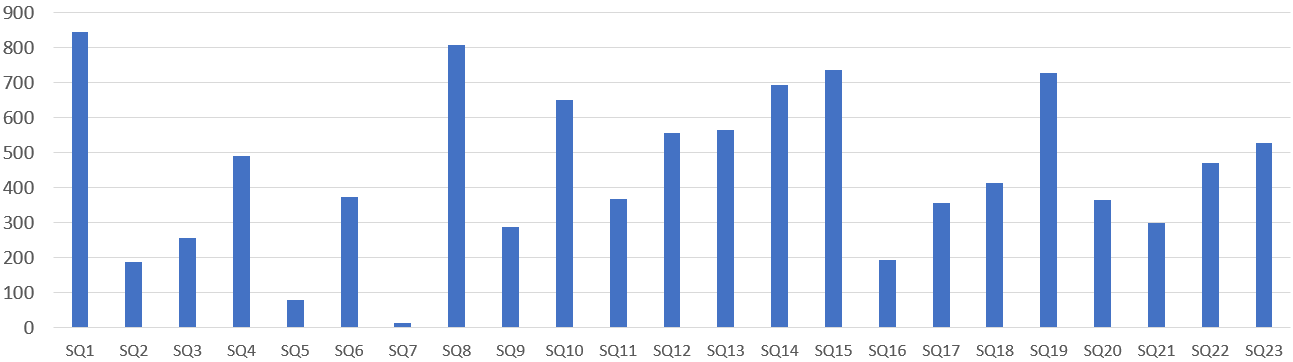
\includegraphics[width = \textwidth]{Figure/DatabehandlingSkalaer/Varians} 
%%\caption{Søjlediagram over variansen for besvarelserne til hvert Scale Question.}
%%\label{fig:Varians}
%%\end{figure}
%%\noindent
%%
%%Det tydeligt at se ud fra \autoref{fig:Varians} at der er stor forskel mellem variansen ved de forskellige SQ. For eksempel er variansen for SQ5 og SQ7 meget lav i forhold til SQ1 og SQ8. 
%%
\subsection{Standardisering af besvarelser}
Når variansen ikke er ens for ens data kan det i nogle tilfælde vælges at udligne variansen når der skal udføres PCA. Hvis variansen skulle udlignes vil det kræve en standardisering af data. Formålet med at gøre dette er at data med lav varians i rå data får lige betydning i PCA som rå data med stor varians. 

Det vælges ikke at standardisere data, da det kan give skævvridninger, som ikke er ønsket. Testpersonerne har reelt haft muligheden for at svare på hele skalaen, men har valgt at afgive besvarelser i nærheden af hinanden, hvilket tolkes som at de har været mere enige i dette tilfælde end i andre tilfælde hvor der er stor spredning.
\newpage

%Al data er målt med samme måleenhed, da det er målt på samme skala, der går fra 0 til 100 ved aflæsningen. Dette er en del af begrundelsen for ikke at standardisere, da det ofte gøre i tilfælde hvor målingerne ikke er målt med samme måleenhed. \blankline
%
%Hvis der er større variation ved nogle skalabesvarelser, vil de vægte mere i en PCA, men det vurderes at være acceptabelt og ønsket. Det er dog vigtigt at være opmærksom på dette, når resultaterne af PCA analyseres. 
